\title{Generalized Analytic Microburst Model Report}
\author{Mike Shumko}
\date{\today}

\documentclass[12pt]{article}
\usepackage{graphicx}
\begin{document}
\maketitle

I looked for and found an elegant way to calculate the analytic microburst CDF that is generalized to any microburst PDF distributions. The geometry of the analytic model is shown in Fig. \ref{fig_diagram} and the basic idea is that given an AC6 separation $s$ and microburst radius $r$, there exists a circular area of radius $r$ around each spacecraft where these microbursts will be observed by either spacecraft. Furthermore as Fig. \ref{fig_diagram}B and C show, if the ratio of $r$ and $s$ is such that the circular area around each spacecraft overlap, the overlapping area contains all possible microburst center locations that will be simultaneously observed. The area of the overlapping circles can be found using the special case of the circle-circle intersection formula\footnote{http://mathworld.wolfram.com/Circle-CircleIntersection.html}

\begin{equation}
A(r, s) = 2 r^2 \cos^{-1} \Bigg( \frac{s}{2r} \Bigg)- \frac{s}{2} \sqrt{4 r^2 - s^2}
\end{equation}

Now we need to derive an expression of how $A(r, s)$ changes as a function of spacecraft separation. To compare this to the AC6 results, we will need to calculate the microburst CDF, $F(s)$. $F(s)$ can be interpreted as the fraction of microbursts that was observed above a separation $s$ and is technically a complementary CDF. We will first derive a simple case of a single size microburst population and then generalize it to a continuous distribution of microburst sizes.

\begin{figure}
\includegraphics[width=\textwidth]{analytic_microburst_model_diagram.png}
\caption{The geometry of the analytic model showing the locations of all possible microburst centers that can be observed by one or both AC6 units as a function of microburst radius $r$ and AC6 separation $s$. The two AC6 units are shown as black dots and the enclosing black circle bounds the area where a microburst will be observed by one or both AC6 units if its center lies inside the circle. Panel (A) shows the case where microburst diamater is smaller than the AC6 separation ($2r < s$). In this scenario all microbursts will be observed by either unit A or B and never simulatenously. Panel (B) shows the intermediate case where the microburst diameter is comporable to the AC6 separation ($2r \approx s$) and some fraction of microbursts will be observed simulatenously. The area contaning the centers of microbursts observed by both spacecrraft is the circle intersection and is highlighted with gray shading. Lastly, panel (C) shows the case where the spacecraft separation is much smaller than the microburst size ($r >> s$) and nearly all microbursts observed by one unit will also be observed by the other.} \label{fig_diagram}
\end{figure}

\section{Single-size microburst distribution}
For a direct comparison with $F(s)$ derived from the AC6 data we have to integrate $A(r_0, s)$ over all separations above $s$ and normalize such that $F(0) = 1$. Assuming a fixed-microburst population with a radius $r_0$, $F(s)$ is given by

\begin{equation}
F(s) = \frac{\displaystyle\int\displaylimits_{s}^{\inf} A(r_0, s') ds'}{\displaystyle\int\displaylimits_{0}^{\inf} A(r_0, s') ds'}
\end{equation} where the primed variables are dummy integration variables.

\end{document}